\documentclass[tikz]{standalone}
\usepackage{tikz}
\usetikzlibrary{positioning, graphs}
\usetikzlibrary{graphs.standard}
\usetikzlibrary{arrows.meta}
\begin{document}
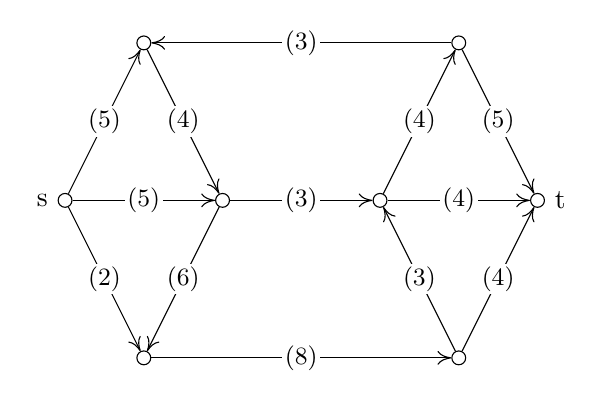
\begin{tikzpicture}
	[vertex/.style={draw,circle,inner sep = 0em, minimum size = 0.5em, fill=white},
		 edgelabel/.style = {fill = white, inner sep = 0.1em, font=\small}]
	\node[vertex, label = left : s] (s) at (0, 0) {};
	\node[vertex] (a) at (1, 2) {};
	\node[vertex] (b) at (5, 2) {};
	\node[vertex] (c) at (2, 0) {};
	\node[vertex] (d) at (4, 0) {};
	\node[vertex] (e) at (1, -2) {};
	\node[vertex] (f) at (5, -2) {};
	\node[vertex, label = right : t] (t) at (6, 0) {};
	
	\draw[-{>[length=5, width=5]}] (s) to node[edgelabel] {$(5)$} (a);
	\draw[-{>[length=5, width=5]}] (s) to node[edgelabel] {$(5)$} (c);
	\draw[-{>[length=5, width=5]}] (s) to node[edgelabel] {$(2)$} (e);
	\draw[-{>[length=5, width=5]}] (a) to node[edgelabel] {$(4)$} (c);
	\draw[-{>[length=5, width=5]}] (b) to node[edgelabel] {$(3)$} (a);
	\draw[-{>[length=5, width=5]}] (b) to node[edgelabel] {$(5)$} (t);
	\draw[-{>[length=5, width=5]}] (c) to node[edgelabel] {$(3)$} (d);
	\draw[-{>[length=5, width=5]}] (c) to node[edgelabel] {$(6)$} (e);
	\draw[-{>[length=5, width=5]}] (d) to node[edgelabel] {$(4)$} (b);
	\draw[-{>[length=5, width=5]}] (d) to node[edgelabel] {$(4)$} (t);
	\draw[-{>[length=5, width=5]}] (e) to node[edgelabel] {$(8)$} (f);
	\draw[-{>[length=5, width=5]}] (f) to node[edgelabel] {$(3)$} (d);
	\draw[-{>[length=5, width=5]}] (f) to node[edgelabel] {$(4)$} (t);
\end{tikzpicture}
\end{document}